%%
%% This is file `sample-sigconf.tex',
%% generated with the docstrip utility.
%%
%% The original source files were:
%%
%% samples.dtx  (with options: `sigconf')
%% 
%% IMPORTANT NOTICE:
%% 
%% For the copyright see the source file.
%% 
%% Any modified versions of this file must be renamed
%% with new filenames distinct from sample-sigconf.tex.
%% 
%% For distribution of the original source see the terms
%% for copying and modification in the file samples.dtx.
%% 
%% This generated file may be distributed as long as the
%% original source files, as listed above, are part of the
%% same distribution. (The sources need not necessarily be
%% in the same archive or directory.)
%%
%% The first command in your LaTeX source must be the \documentclass command.
\documentclass[sigconf, nonacm]{acmart}

%%
%% \BibTeX command to typeset BibTeX logo in the docs
\AtBeginDocument{%
  \providecommand\BibTeX{{%
    \normalfont B\kern-0.5em{\scshape i\kern-0.25em b}\kern-0.8em\TeX}}}

%%
%% end of the preamble, start of the body of the document source.
\begin{document}

%%
%% The "title" command has an optional parameter,
%% allowing the author to define a "short title" to be used in page headers.
\title{Using Machine Learning to Analyze NFL Penalty Data}

%%
%% The "author" command and its associated commands are used to define
%% the authors and their affiliations.
%% Of note is the shared affiliation of the first two authors, and the
%% "authornote" and "authornotemark" commands
%% used to denote shared contribution to the research.

\author{Leo DiPerna}
\affiliation{%
  \institution{Virginia Tech}
  \city{Blacksburg}
  \state{Virginia}
}
\email{dipernalz@vt.edu}

\author{Eric Uehling}
\affiliation{%
  \institution{Virginia Tech}
  \city{Blacksburg}
  \state{Virginia}
}
\email{uehlingeric@vt.edu}

%%
%% By default, the full list of authors will be used in the page
%% headers. Often, this list is too long, and will overlap
%% other information printed in the page headers. This command allows
%% the author to define a more concise list
%% of authors' names for this purpose.
\renewcommand{\shortauthors}{DiPerna and Uehling}

%%
%% A "teaser" image appears between the author and affiliation
%% information and the body of the document, and typically spans the
%% page.
\begin{teaserfigure}
  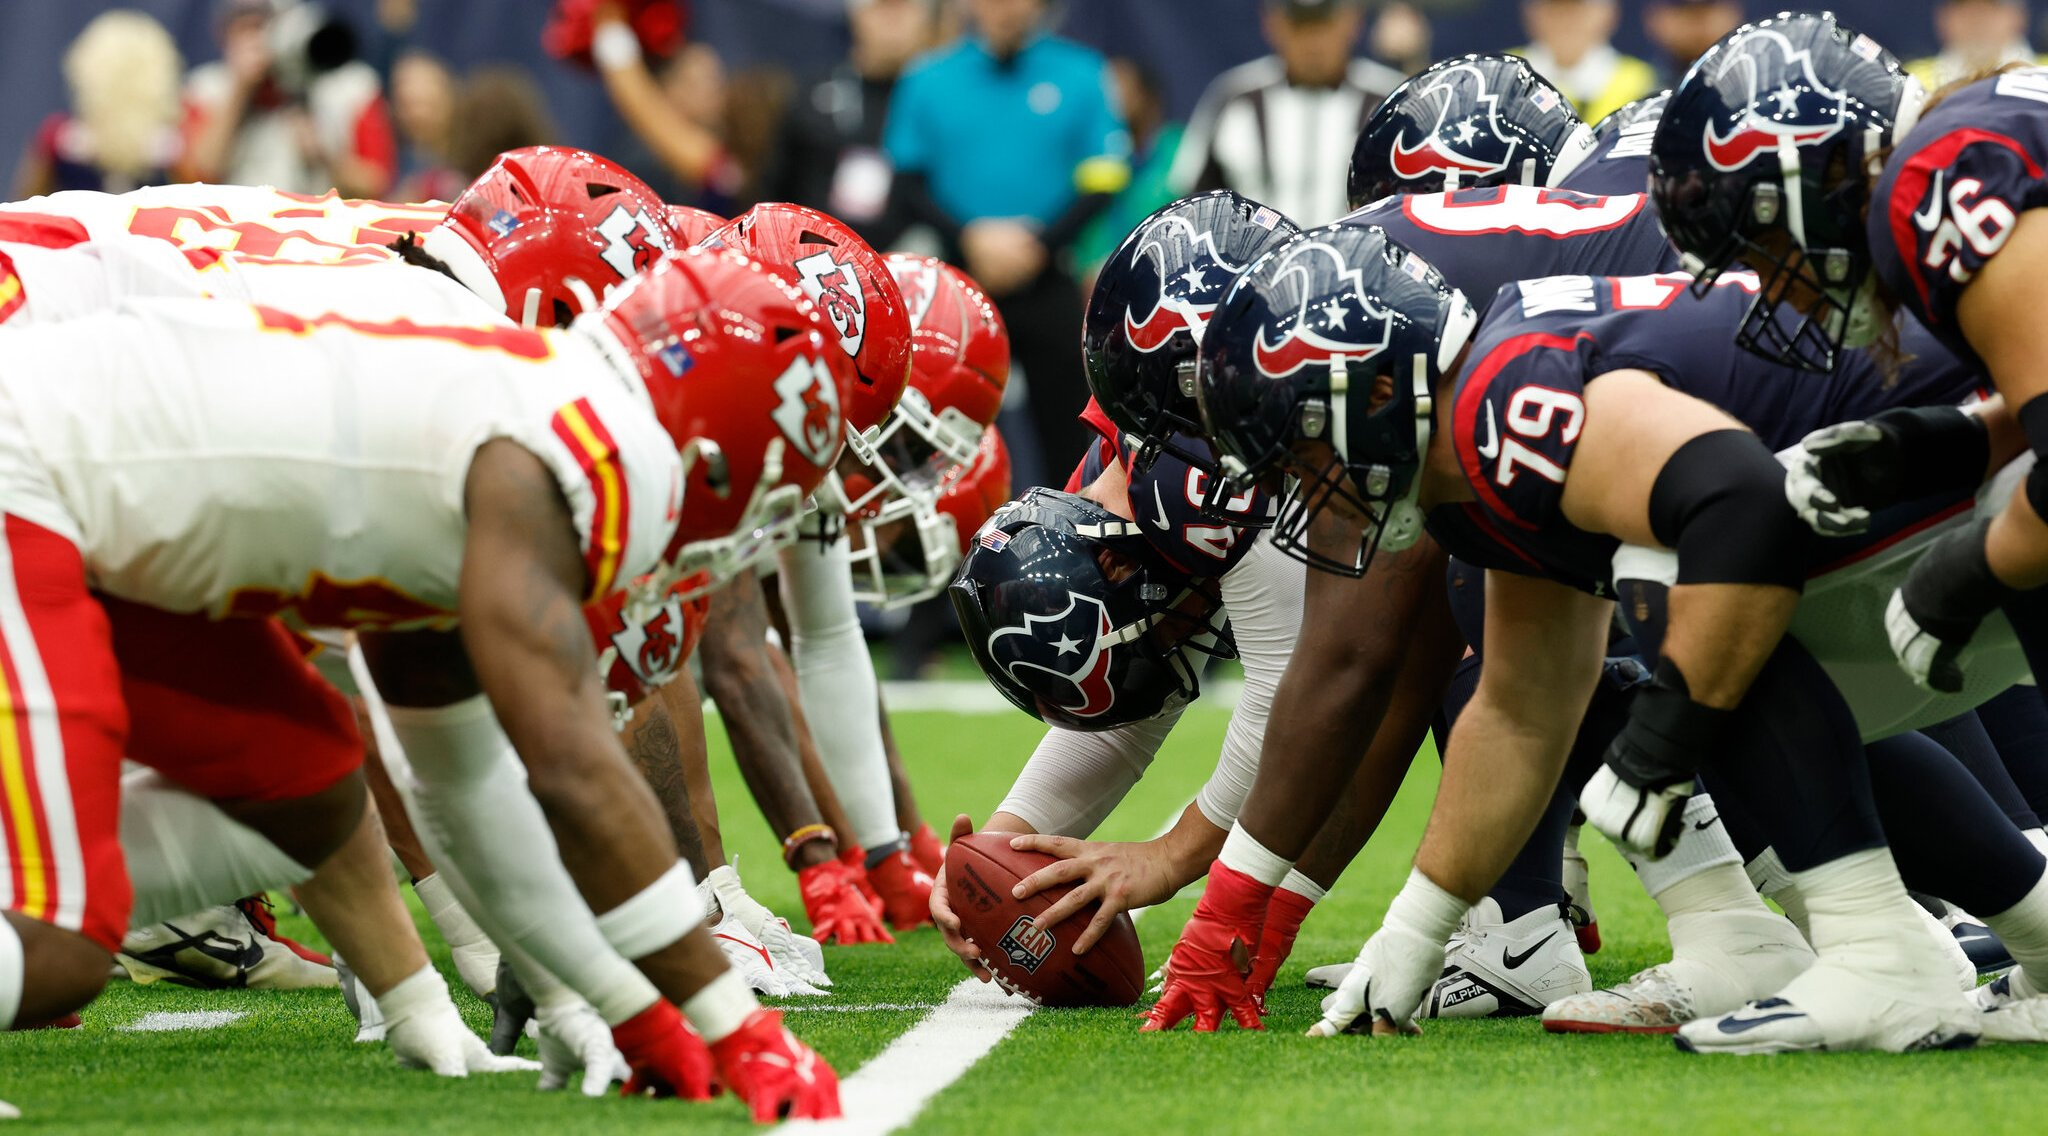
\includegraphics[width=\textwidth]{images/football_picture}
  \caption{Players for the Kansas City Chiefs and Houston Texans lining up for a
           play during an NFL game \cite{NYTImage}.}
  \label{fig:teaser}
\end{teaserfigure}

%%
%% This command processes the author and affiliation and title
%% information and builds the first part of the formatted document.
\maketitle

\section{Introduction}

Which NFL penalties have the biggest impact on the results of drives, or on the
results of games or on the outcomes of seasons? Which referees tend to call
which penalties? Is it possible to predict the outcome of drives given the
penalties that occurred during that drive? Is it possible to predict the
penalties that a specific referee crew will call?

As avid NFL fans, these are the types of questions that we aimed to answer to
gain a deeper insight into the effect that NFL penalties have on the league.
NFL fans know that penalties have a big impact on the outcome of games, but are
less sure about the specifics of their impact.

We were able to create a regression model that predicts the points scored during
a drive given the the number of offensive and defensive penalties and the number
of penalty yards from those penalties. This model used a gradient boosting
regressor. We were also able to create a generalized linear model that predicted
the number of each type of penalty that a referee crew called during a game.
% TODO: add a sentence for each of the other models

We believe that we were able to uncover insights that fans, teams, and analysts
of the game will all find useful and interesting.

\section{Previous Work}

Before beginning to analyze our data, we looked at a number of previous papers
that analyzed NFL data so that we had the necessary background and context to 
develop our own methods. We will provide a brief overview of the most
important works that we looked at.

Researchers at University North in Croatia \cite{Tomislav20} looked at a wide
range of previous research in sport outcome prediction and provided a broad
overview of techniques that are being looked at. The papers that they looked
at encompassed a wide range of sports, including NFL, NBA, and various
international soccer leagues. They found that the most of these papers used some
sort of feature selection or feature extraction algorithm prior to using an ML
algorithm, which was most often neural networks. They also found that most
researchers decided to treat the problem of outcome prediction as a
classification problem.

Researchers at the University of Port Harcourt in Nigeria \cite{Anyama15}
attempted to use neural networks in combination with linear regression to
predict the results of NFL games. They used linear regression to choose features
from their dataset and then used those features to train a neural network. This
gave us some insight into creative ways that we could select features when
training our models.

Students at Denison University \cite{Blaikie11} attempted to use neural networks
to predict the results of NFL games. They
made a number of different models which selected different sets of features and
trained their models based on these sets of features. For example, one set of
features that they used comprised only of basic statistics such as passing
yards, rushing yards, points, and turnovers. They derived another set of
features using principal component analysis to reduce a large set of features to
a smaller set. This gave us some more insight into how we could select features
when training our models.

Researchers at Texas Tech University \cite{Craig16} investigated how the
ambient temperature during NFL games resulted in more aggression from players.
They measured aggression by classifying certain penalties as being agressive
penalties and looking at how many of those penalties were committed during a
given game. This gave us some preliminary ideas on ways that we could analyze
and gain insights from penalty data.

A master's student at the University of Iowa \cite{McDaniel21} examined NFL
penalties over the last 20 years in an effort to gain a greater understanding of
the effect of individual referees, the difference between penalty calls against
different NFL teams, and changes in penalties over time. He found that that
there were some major changes in the frequency of penalty calls over time, and
certain seasons where there were noticeably less and noticeably more penalties
called. However, he was also able to determine that these variations were more
due to rule changes and organizational changes rather than the decisions of
individual referees.

Researchers at Skidmore College \cite{Snyder15} examined how consistently
certain penalties are called during different phases of an NFL game. They
examined the frequency of penalties at different times during the game and also
looked at the status of the game of the game as it related to the frequency of
penalty calls. They found that judgement penalty calls varied considerably
depending on the status of the game. These penalties were called less frequently
than expected during the first five and last five minutes of the game.

\section{Feature Preparation}

This project consisted of three steps: data collection, data cleaning, and data
analysis. We will discuss the data collection and data cleaning processes in
this section as well as some of the preliminary data exploration that we did.
We will go into the specifics of our data analysis in the next section.

\subsection{Collection}

To be able to conduct a full analysis of the impact of penalties on different
facets of the NFL, we needed to collect a wide range of data from NFL games.
The data that we collected includes a dataset of individual penalties, a dataset
of drive results, a dataset of game results, a dataset of season results, and a
couple of miscellaneous dataset to link the others together.

We were unable to find any easily accessible datasets that satisfied all of our
requirements, so we decided to collect our data via web scraping. We scraped
data from Pro Football Reference, a website that provides a massive amount of
NFL statistics dating back to the start of the league. We decided to collect
data starting from the 2009 season and continuing to the present.

Pro Football Reference has a webpage for every NFL game. This webpage contains
tons of information about every game, including the results of each drive,
statistics for each player, and the results of each play. Each webpage has the
same format, and the URL of each webpage had a predictable format. This allowed
us to create a web scraping script that could systematically generate a link for
each game from 2009 to the present, read the data from each table in the
webpage, and output the important data to CSV files. Using this script, we were
able to collect data on drive results and game results.

However, we still needed to collect data on penalties. To collect penalty data,
we used a different website, nflpenalties.com. This site contains a page for
each season-team combination that lists all penalties that the team committed in
that season in a table. By scraping this site, we were able to create a dataset
that contains every penalty committed by every team from 2009 to the present.

\subsection{Data Cleaning}

After scraping the data, we needed to do some data cleaning to prepare the
features that we wanted for model training. The raw data files that we used
were:

\begin{itemize}
  \item \verb|drives.csv| -- Contains a row for every drive that occurred during
    our study period.
  \item \verb|penalties.csv| -- Contains a row for every penalty that occurred
    during our study period.
  \item \verb|game_detail.csv| -- Contains a row for every game that occurred
    during our study period.
\end{itemize}

To analyze the effect of penalties on the outcome of drives, we needed to know
which penalties occurred on which drives. This meant that we needed to merge
the data in \verb|drives.csv| with the data in \verb|penalties.csv|. Since each
row in \verb|penalties.csv| contained the time during the game that the penalty
occurred, and each row in \verb|drives.csv| contained the time during the game
that the drive occurred, we were able to get a count of each penalty during each
drive by iterating over each penalty and matching it with its drive.

In the different data files that we collected, there were a number of different
formats for team and game IDs. This made determining which game a drive occurred
in and determining which game a penalty occurred in difficult, so we had to
standardize the format of the game ID column across our dataframes.

There were also some annoying quirks with the data that we had to solve. For
example, the NFL season changed from 16 regular season games to 17 beginning
during the 2021 season. This was in the middle of our study period, so we had
to account for this when determining the week that a game occurred. There are
also a number of teams that changed their names or cities during our study
period, so we also had to account for that and make sure that teams were matched
to the same team ID regardless of whether their name had changed.

We decided to ignore special teams penalties and focus solely on offensive and
defensive penalties, so we had to filter out penalties based on the phase of the
game that they occurred in.

\subsection{Exploratory Data Analysis}

Before deciding which models to make, we did some exploratory data analysis to
gain some insight into the data. Here are some of the most interesting insights
that we were able to gain from looking at the data.

\begin{figure}[h]
  \centering
  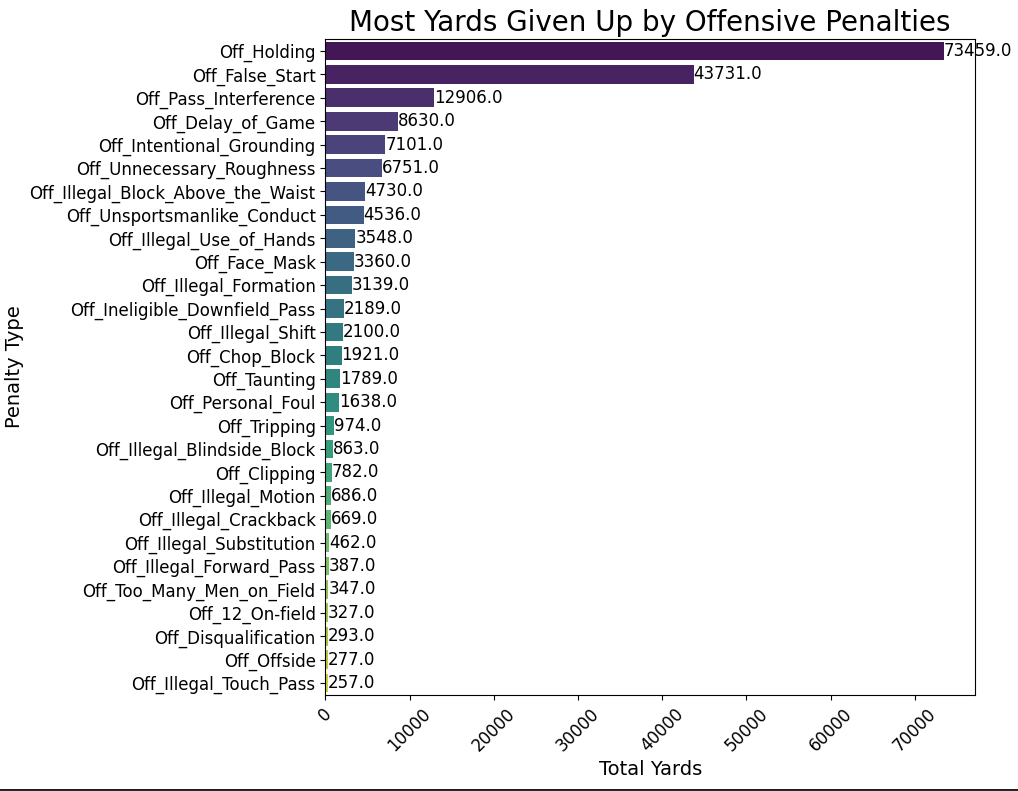
\includegraphics[width=\linewidth]{images/eda_3.png}
  \caption{Penalty yardage by offensive penalties.}
\end{figure}

\begin{figure}[h]
  \centering
  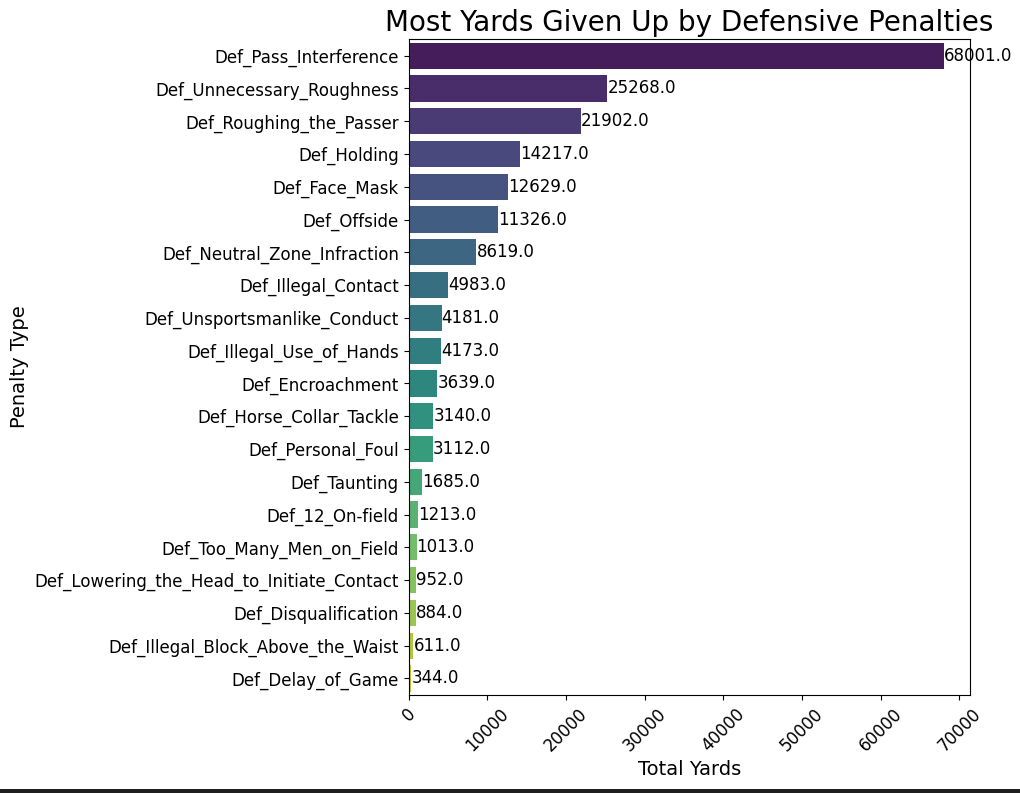
\includegraphics[width=\linewidth]{images/eda_4.png}
  \caption{Penalty yardage by defensive penalties.}
\end{figure}

From these graphs, we can see that certain penalties have a much larger impact
on the outcomes of games than others. On the offensive side, holding and false
starts seem to have a much bigger impact than all of the other penalties
combined. On the defensive side, defensive pass interference has a much larger
impact than any other penalty, which makes sense because it is a spot foul that
can cost a team an unlimited number of yards.

\begin{figure}[h]                                                               
  \centering
  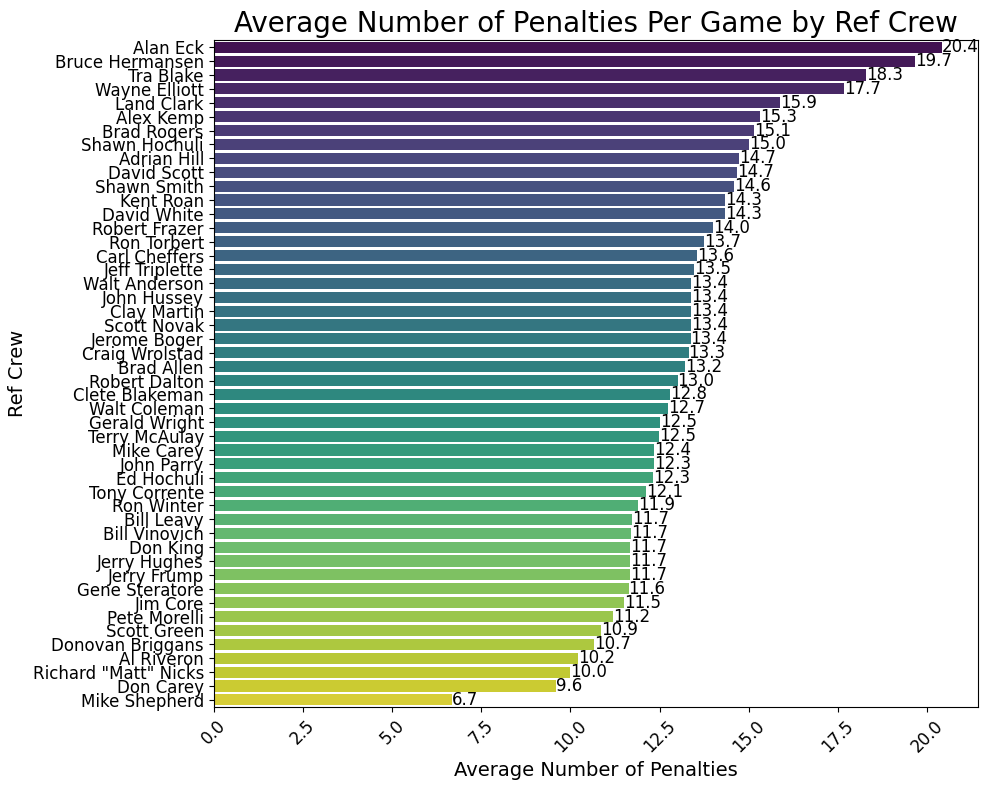
\includegraphics[width=\linewidth]{images/eda_1.png}
  \caption{Average number of penalties called per game by referee crew.}
\end{figure}

We observed that there was a wide range of penalties that each referee crew
called per game. The lowest was Mike Shepherd's crew, which only called an 
average of 6.7 penalties per game. The highest was Alan Eck's crew, which called
20.4 penalties per game. This means that Alan Eck's crew called over three times
as many penalties per game when compared to Mike Shepherd's crew. Such a drastic
discrepancy led us to think that we might be able to predict a different number
of penalties in a game based on the referee crew that was doing that game.

\begin{figure}[h]
  \centering
  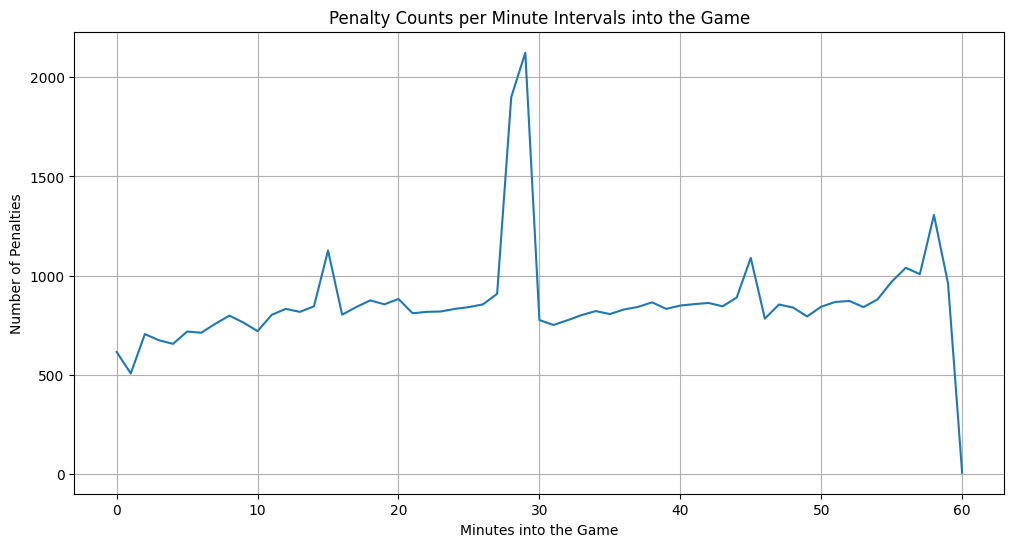
\includegraphics[width=\linewidth]{images/eda_2.png}
  \caption{Distribution of penalties at different times during a game.}
\end{figure}

We also found it interesting that there seemed to be a noticeable difference in
the number of penalties called at different times during a game. It seems like
the number of penalties increases from the beginning of each half to the end of
each half, with a large spike near the end of the half. This spike is larger at
the end of the first half than it is at the end of the second half. This might
indicate that more penalties are called during tense situations than during
normal situations.

\section{Results}

In this section, we will discuss the models that we made, the accuracy of each
model, and what we can learn from each model in the context of football.

TODO: Subsubsection for each model

\section{Conclusion}

TODO: Conclusion and future work

%%
%% The next two lines define the bibliography style to be used, and
%% the bibliography file.
\bibliographystyle{ACM-Reference-Format}
\bibliography{final-report}

\end{document}
\endinput
